Cette étude théorique vise à modéliser le comportement d'un faisceau lumineux traversant un prisme d'indice $n$, 
placé dans l'air ($n_{air} = 1$), 
dans l'approximation de l'optique géométrique. 
En considérant des rayons situés dans un plan de section principale, 
nous établirons les relations fondamentales liant la géométrie du prisme à la déviation lumineuse afin d'isoler les conditions optimales de mesure de l'indice de réfraction.

\begin{figure}[h]
    \centering
    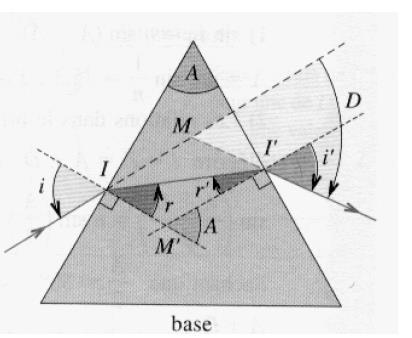
\includegraphics[width=0.7\textwidth]{figures/schema_prisme.jpg}
    \caption{Trajet d'un rayon lumineux en vue du dessus.}
    \label{fig:schema_prisme}
\end{figure}